\chapter{Scenario Series 6-4}

This appendix presents simulation results from the 6-4 scenario series, this tests impact of varying softwood AAC attribution level. 

\section{Summary}
Table \ref{tab:scenario_list} below lists the scenarios in series 6-4. 
Control scenario s6-0 simulates the \emph{status quo} situation (single-level wood supply model with no anticipation of fibre consumption).  

\begin{table}
  \centering
  \begin{tabular}{lll}
    \hline
    Scenario ID & Figure Reference & Description \\
    \hline
    6-0 & \ref{fig:s6-0} & Control scenario. \\
    6-4\_hw100sw110 & \ref{fig:s6-4_hw100sw110} & 110$\%$ of softwood AAC allocated. \\
    6-4\_hw100sw105 & \ref{fig:s6-4_hw100sw105} & 105\% of softwood AAC allocated. \\
    6-4\_hw100sw100 & \ref{fig:s6-4_hw100sw095} & 100$\%$ of softwood AAC allocated\footnote{Identical to scenario 6-1\_p30a01.}. \\
    6-4\_hw100sw095 & \ref{fig:s6-4_hw100sw095} & 95$\%$ of softwood AAC allocated. \\
    6-4\_hw100sw090 & \ref{fig:s6-4_hw100sw090} & 90\% of softwood AAC allocated. \\
    6-4\_hw100sw080 & \ref{fig:s6-4_hw100sw080} & 80\% of softwood AAC allocated. \\
    6-4\_hw100sw060 & \ref{fig:s6-4_hw100sw060} & 60\% of softwood AAC allocated. \\
    \hline
  \end{tabular}
  \caption{Description of scenarios in series 6-4.}
  \label{tab:scenario_list}
\end{table}

\section{Results}

Figures \ref{fig:s6-4_hw100sw100} to \ref{fig:s6-4_hw100sw060} present
simulation results for fifteen scenarios. % Table \ref{tab:scenarios}
% summarizes scenario parameters used in the experiment for each
% scenario.
Disposition of figures is identical for all scenarios. The
first subfigure (a) for each scenario shows the initial
(ie. iteration-0) AAC solution. The second subfigure (b) for each
scenario shows first period of AAC solution for all 30 planning
iterations. The third subfigure (c) for each scenario shows the
implemented harvest level for all 30 planning iterations. Scenarios
3.1 and 3.2 also show profit in this subfigure on a secondary
axis. The fourth subfigure (d) for each scenario shows the difference
between initial and re-planned AAC. The fifth subfigure (e) for each
scenario shows the difference between re-planned AAC and harvest.  The
sixth subfigure (f) for each scenario shows the difference between
initial AAC and harvest. Softwood volume is shown with white bars,
hardwood volume with black bars, and total volume with small
circles. Profit (where applicable) is shown with the $\times$
symbol. 

Hardwood AAC attribution level is kept constant at 100\% for all scenarios. 
As might be expected, softwood attribution levels above 100\% of AAC show more variability in harvest levels and profit, compared to lower-attribution scenarios.
However, impact of over-attributing softwood is relatively low. This may be due to limited availability of pure softwood stands, forcing agent to harvest mixed stands, which in turn saturates the hardwood line.

We can observe declining profit and AAC at, and well below, 100\% softwood AAC attribution level. 
In fact, softwood attribution must be limited to 60\% of AAC to stabilise harvest level and profit over all 30 rolling-horizon replanning cycles.


\begin{figure}[h]
  \centering
  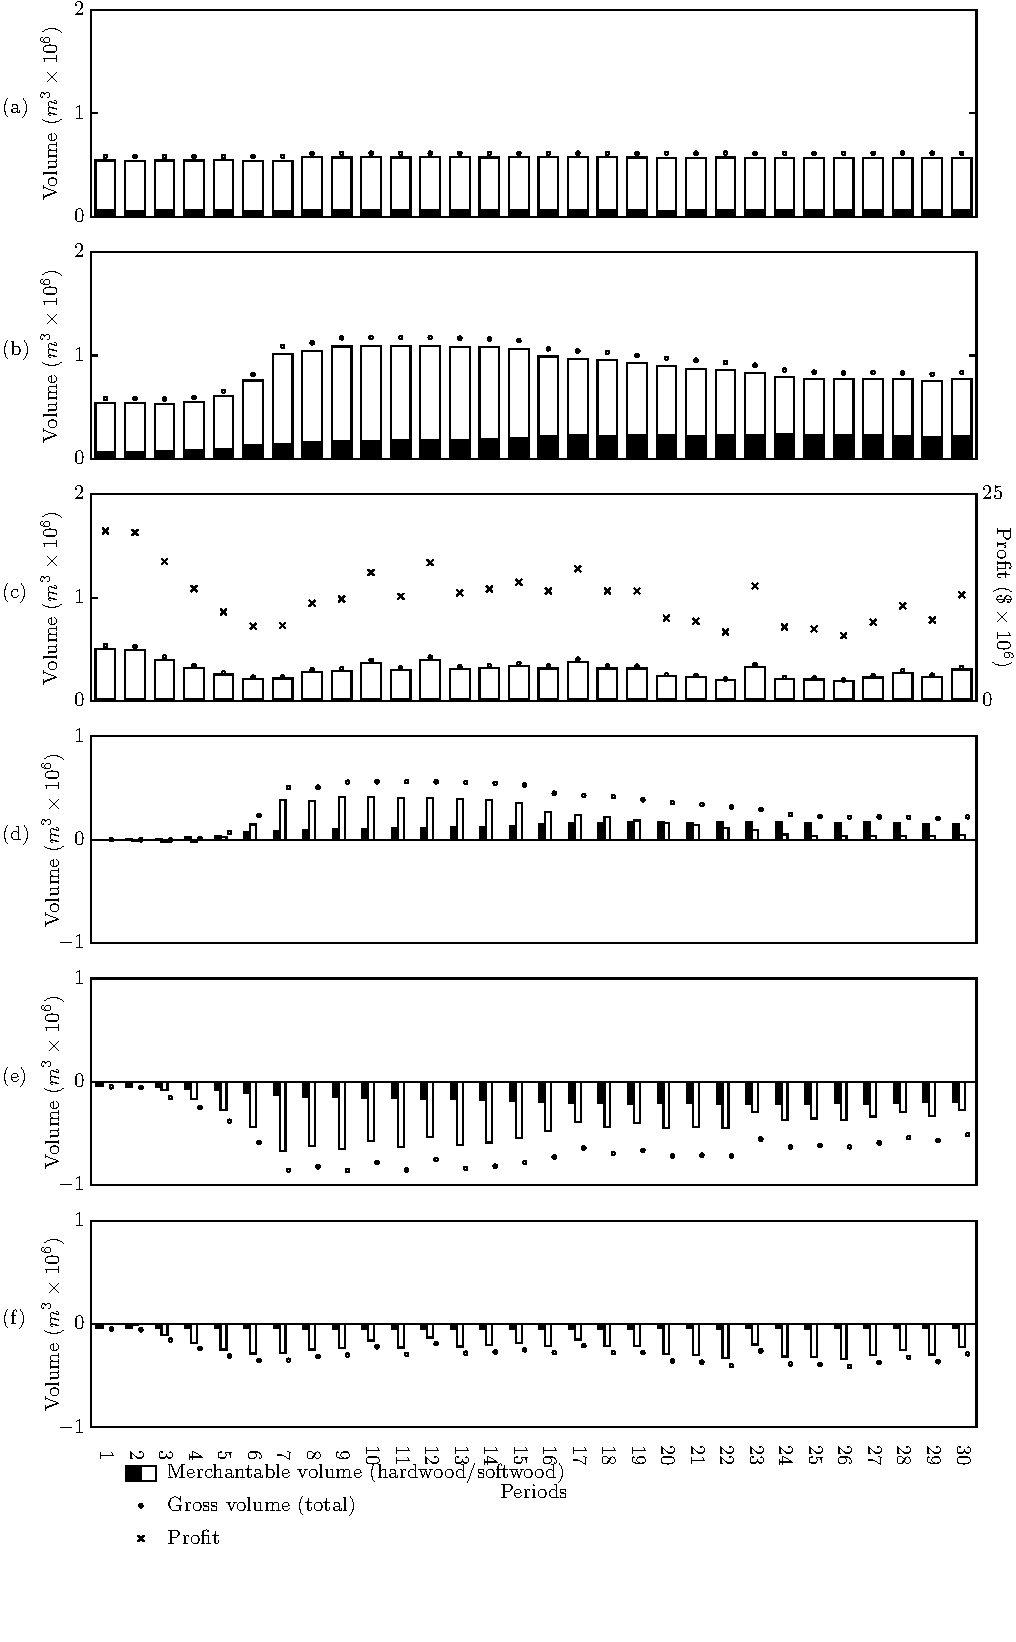
\includegraphics[width=10cm]{images/appendix/s6-0}
  \caption{Scenario 6-0 (control scenario, simulates \emph{status quo}).}
  \label{fig:s6-0}
\end{figure}


\begin{figure}[h]
  \centering
  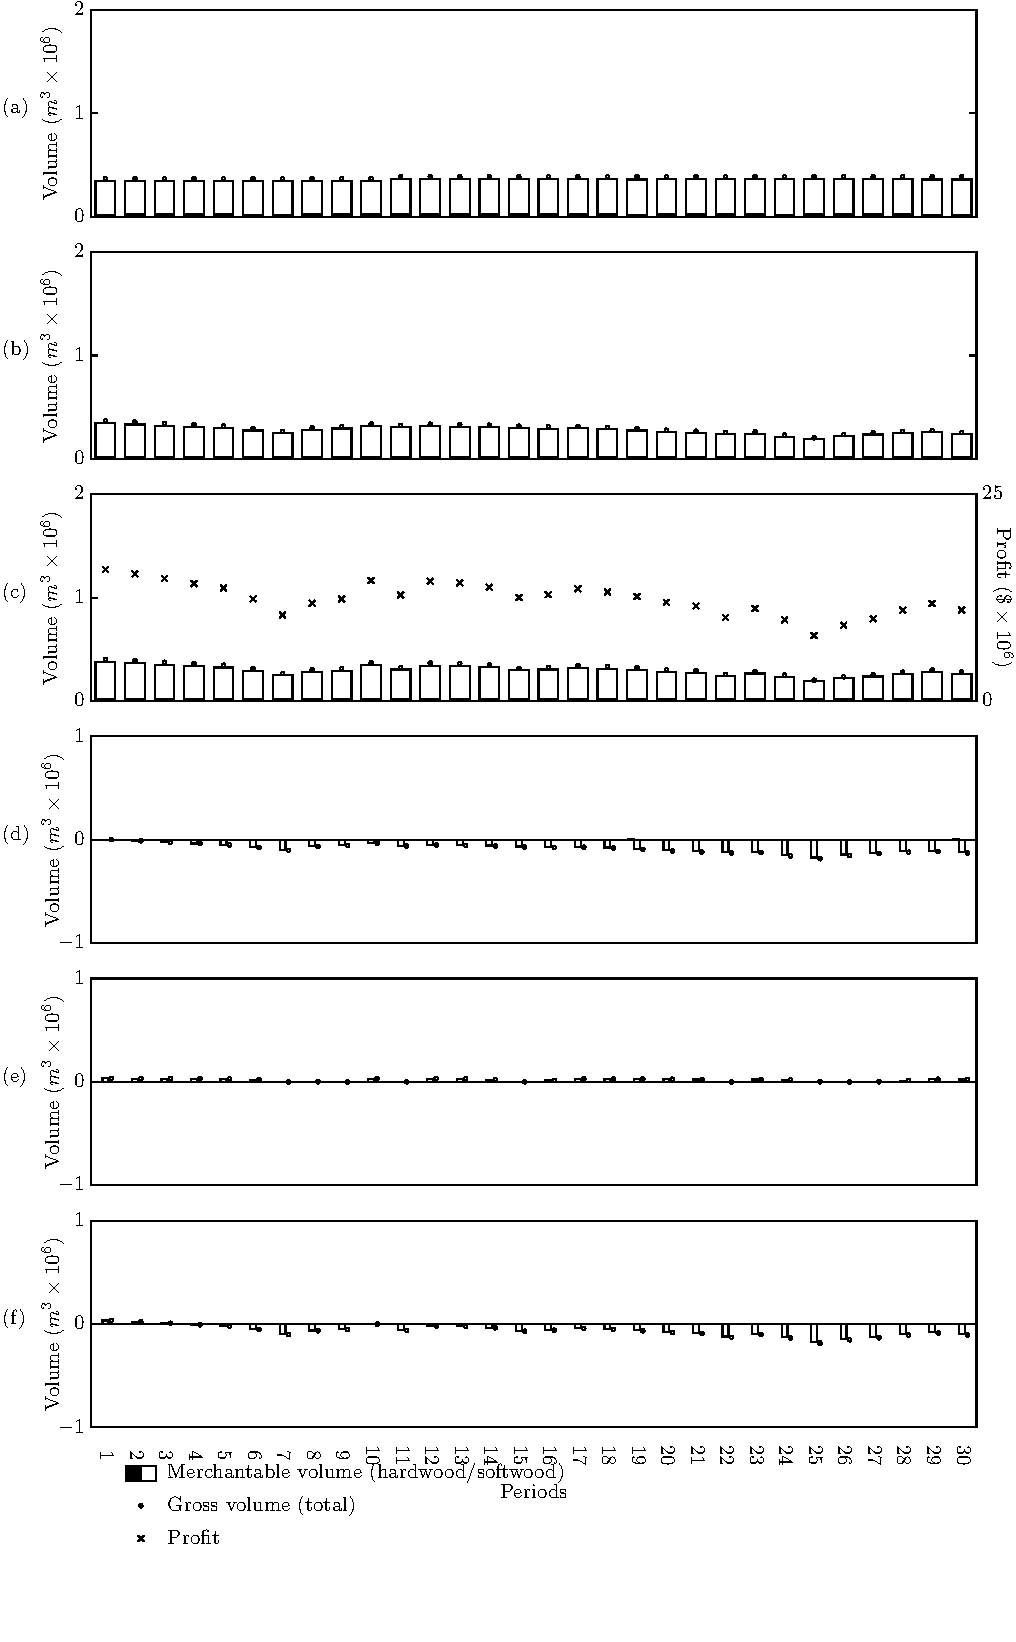
\includegraphics[width=10cm]{images/appendix/s6-4_hw100sw110}
  \caption{Scenario 6-4\_hw100sw110 (110\% of softwood AAC allocated).}
  \label{fig:s6-4_hw100sw110}
\end{figure}

\begin{figure}[h]
  \centering
  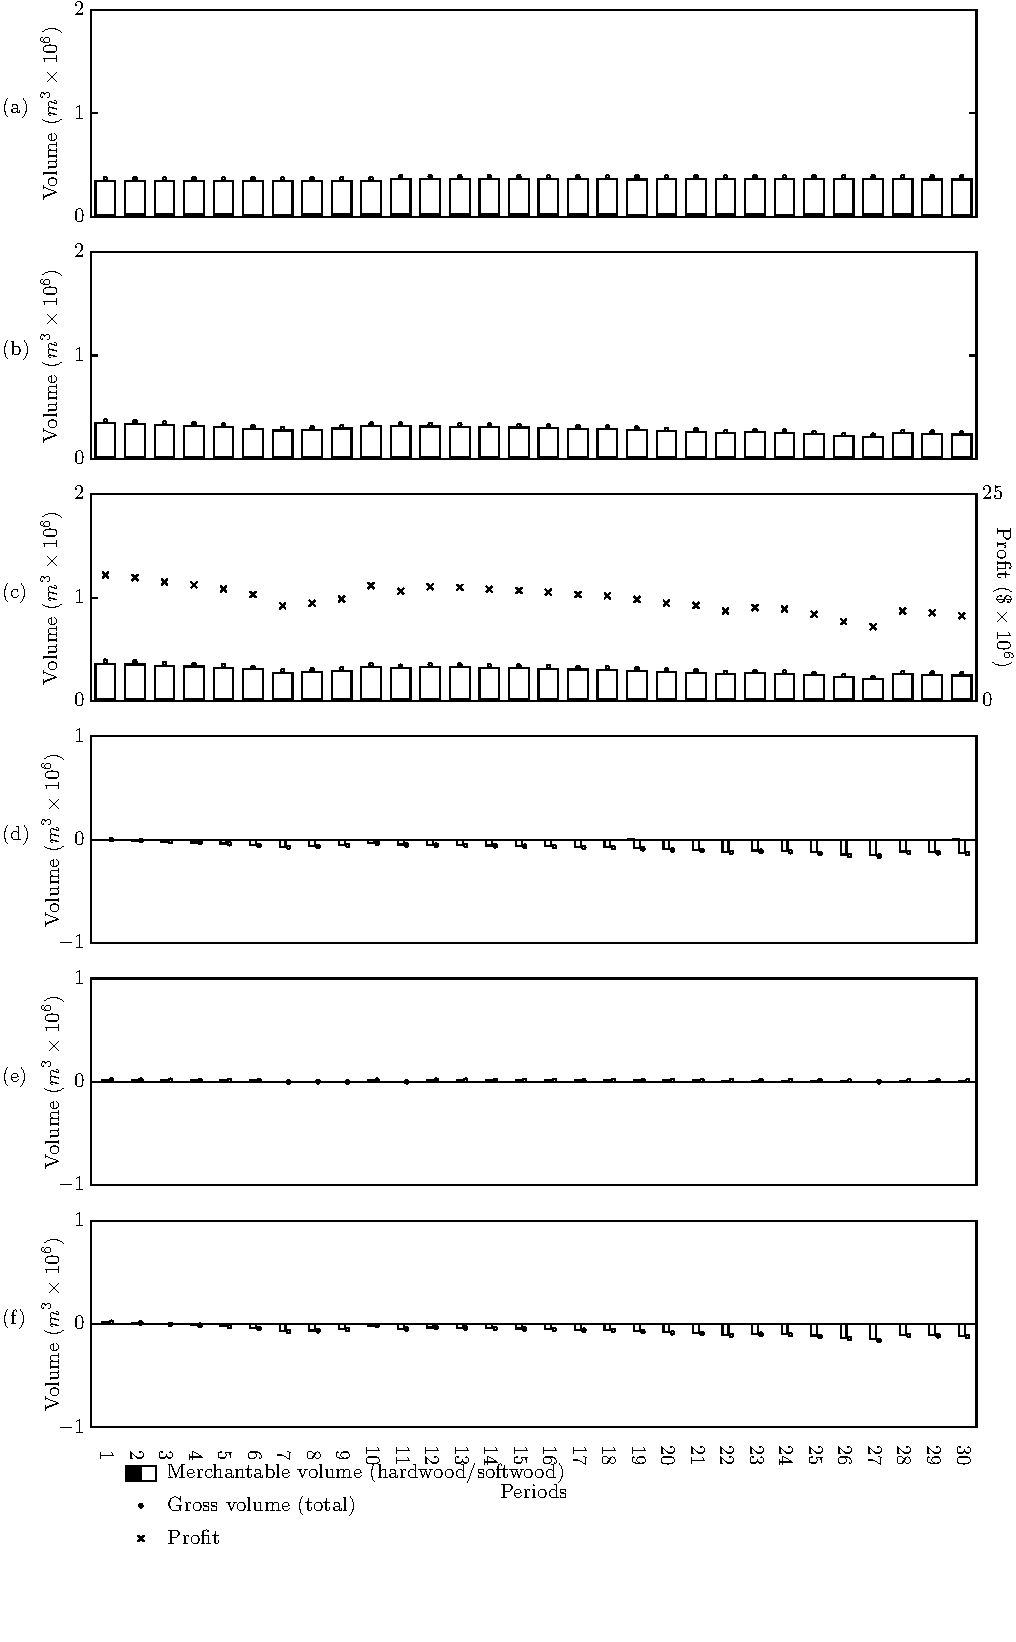
\includegraphics[width=10cm]{images/appendix/s6-4_hw100sw105}
  \caption{Scenario 6-4\_hw100sw105 (105\% of softwood AAC allocated).}
  \label{fig:s6-4_hw100sw105}
\end{figure}

\begin{figure}[h]
  \centering
  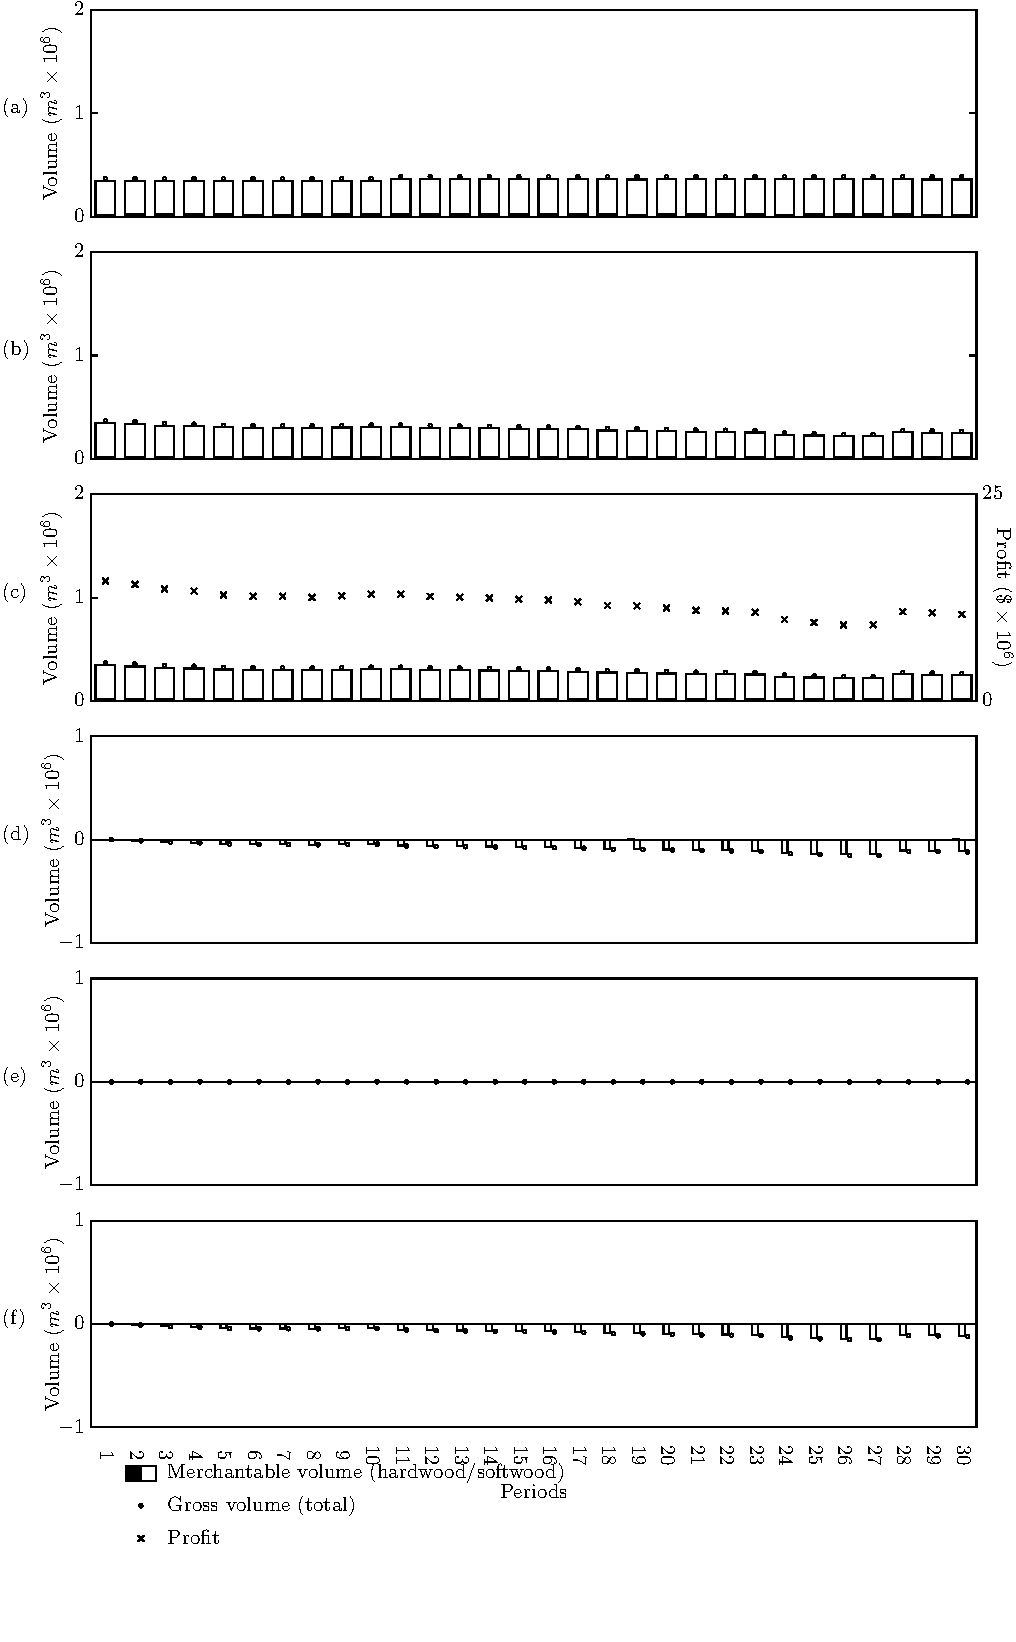
\includegraphics[width=10cm]{images/appendix/s6-1_p30a01}
  \caption{Scenario 6-4\_hw100sw100 (100\% of softwood AAC allocated).}
  \label{fig:s6-4_hw100sw100}
\end{figure}

\begin{figure}[h]
  \centering
  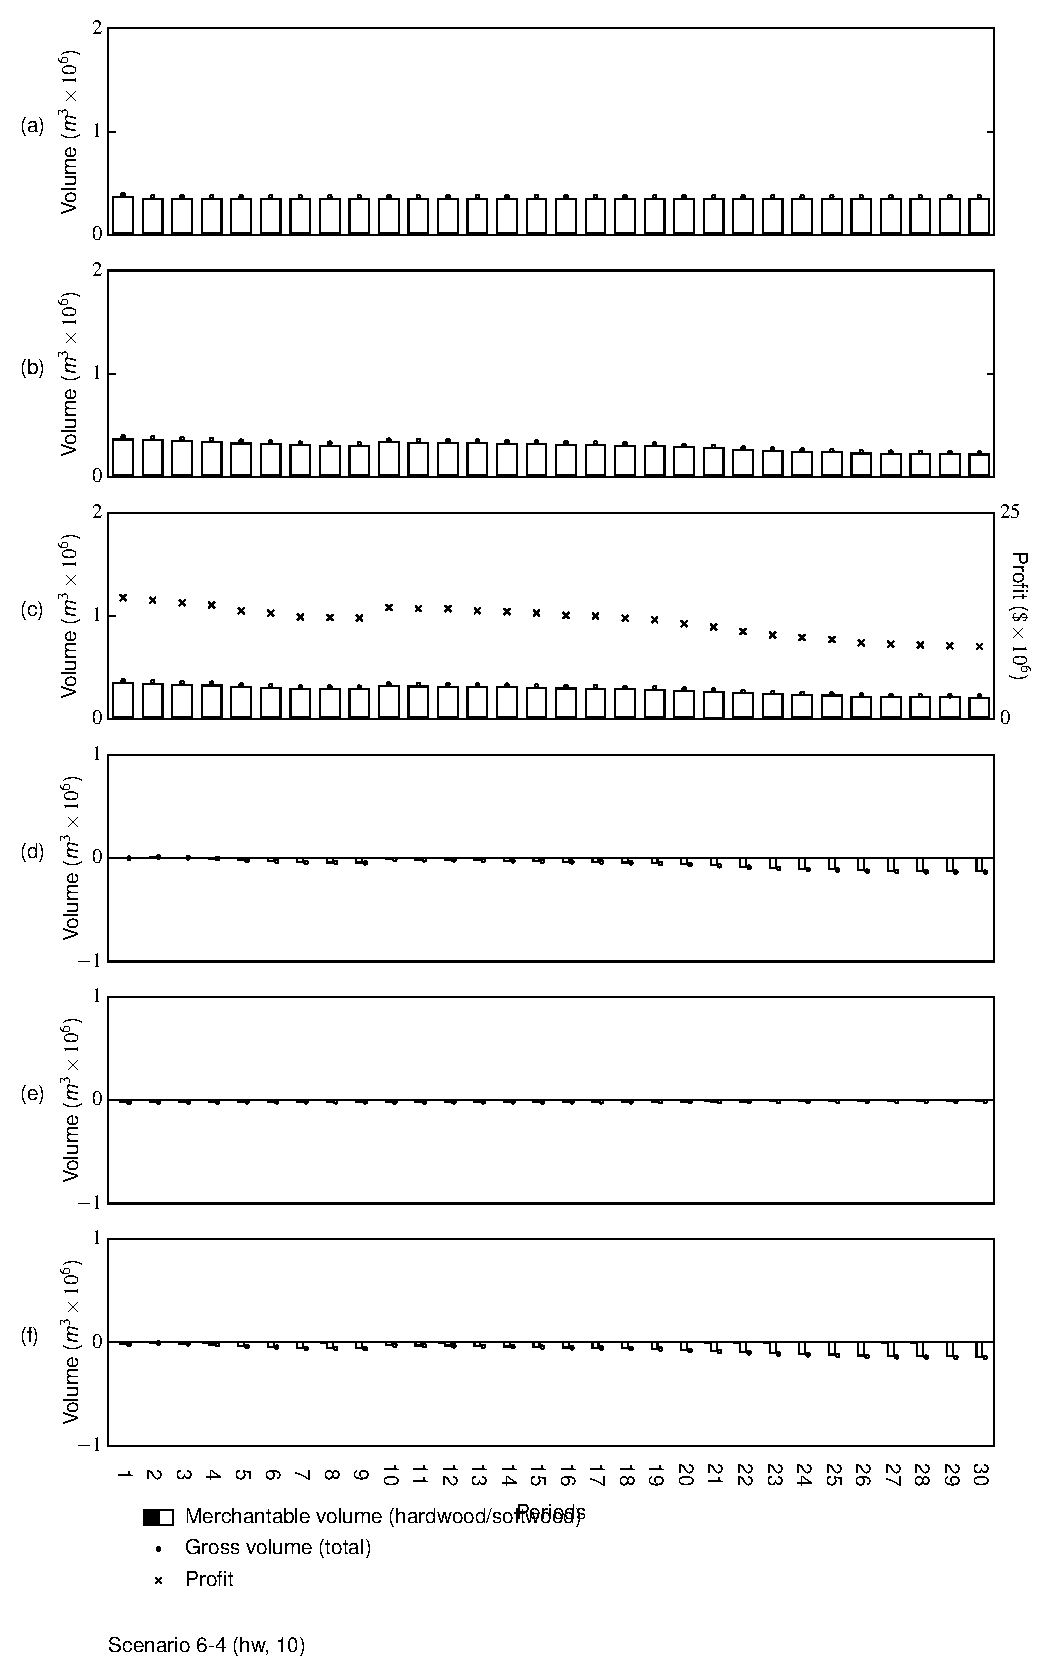
\includegraphics[width=10cm]{images/appendix/s6-4_hw100sw095}
  \caption{Scenario 6-4\_hw100sw095 (95\% of softwood AAC allocated).}
  \label{fig:s6-4_hw100sw095}
\end{figure}

\begin{figure}[h]
  \centering
  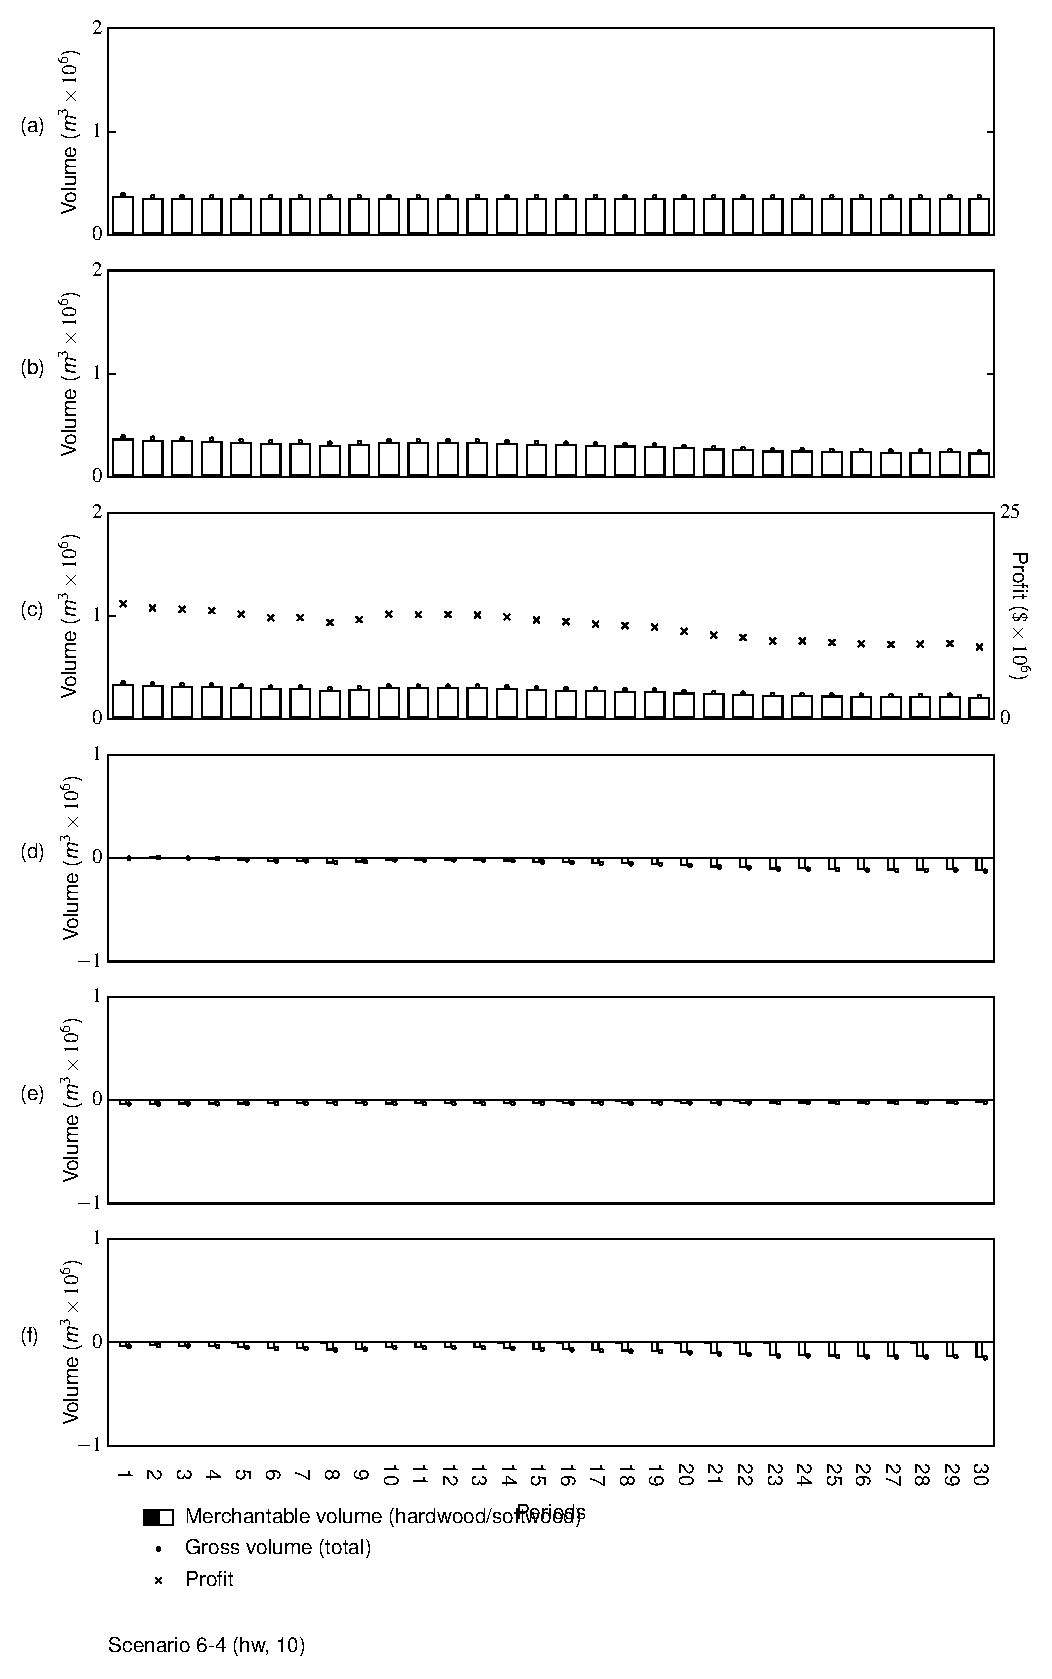
\includegraphics[width=10cm]{images/appendix/s6-4_hw100sw090}
  \caption{Scenario 6-4\_hw100sw090 (90\% of softwood AAC allocated).}
  \label{fig:s6-4_hw100sw090}
\end{figure}

\begin{figure}[h]
  \centering
  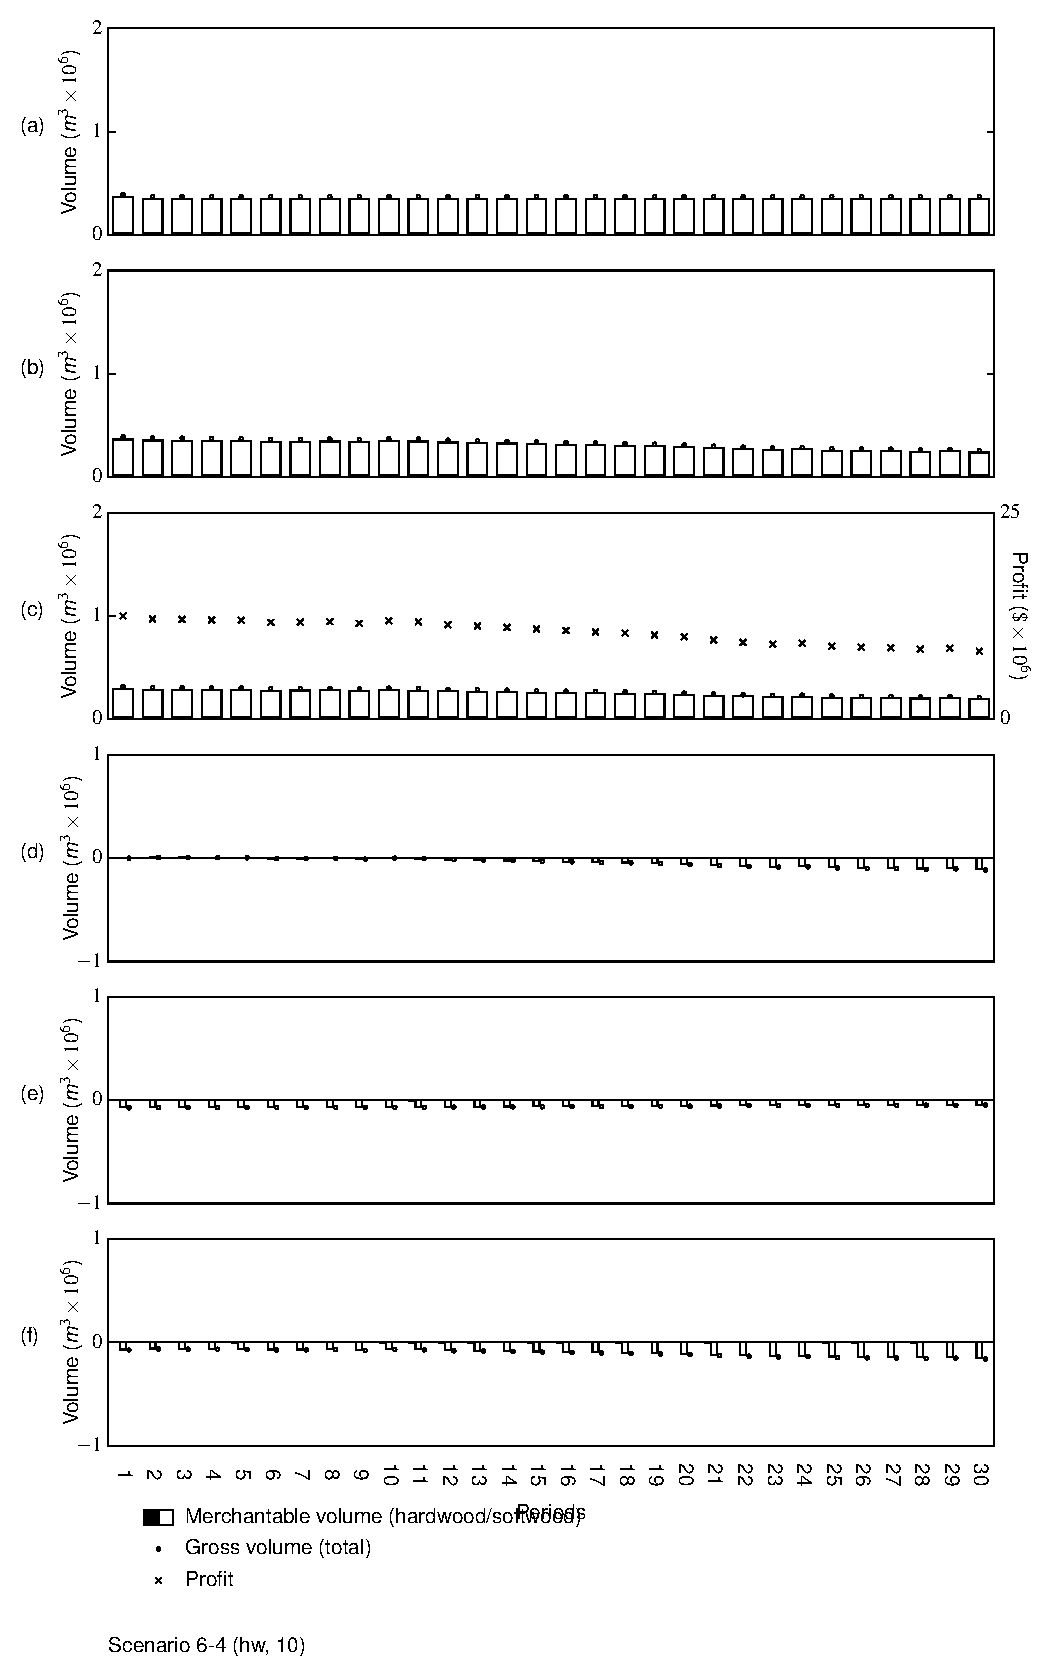
\includegraphics[width=10cm]{images/appendix/s6-4_hw100sw080}
  \caption{Scenario 6-4\_hw100sw080 (80\% of softwood AAC allocated).}
  \label{fig:s6-4_hw100sw080}
\end{figure}

\begin{figure}[h]
  \centering
  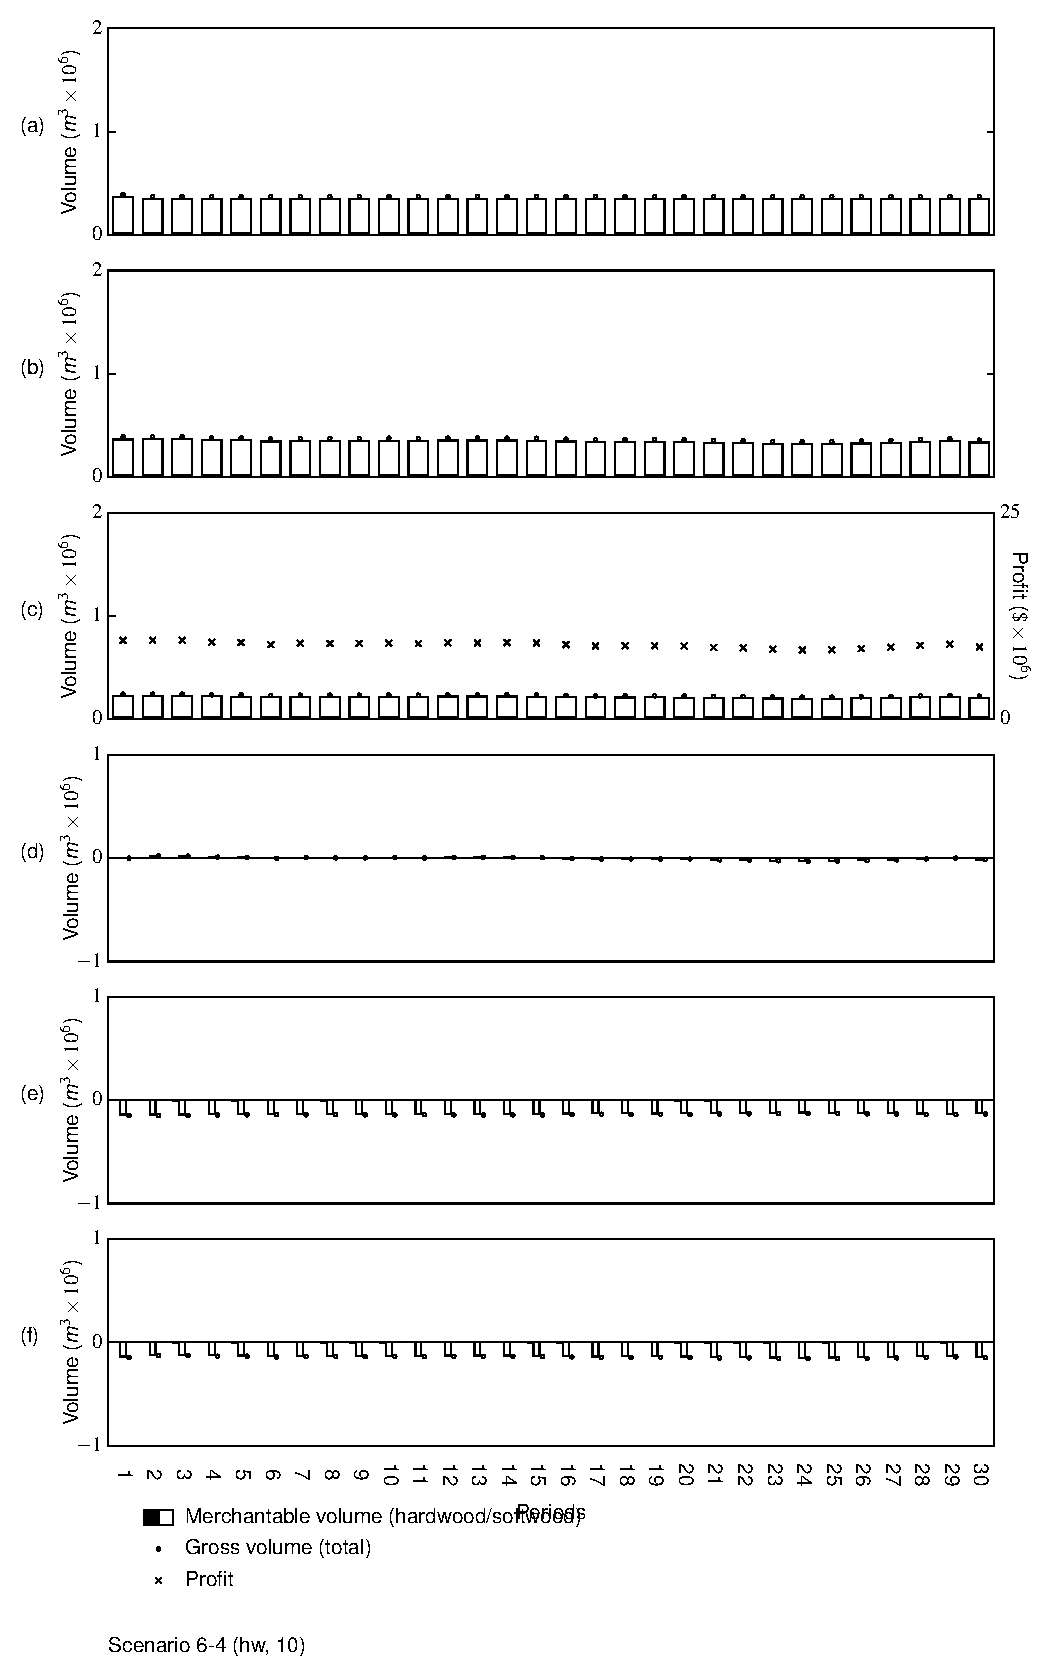
\includegraphics[width=10cm]{images/appendix/s6-4_hw100sw060}
  \caption{Scenario 6-4\_hw100sw060 (60\% of softwood AAC allocated).}
  \label{fig:s6-4_hw100sw060}
\end{figure}
